%include part: see main.beamer.tex and main.article.tex
%include common packages and settings
\usepackage{etex} %эта магическая херь избавляет от переполнения регистров TeX а!!!

\mode<article>{\usepackage{fullpage}}
\mode<presentation>{
    \usetheme{Madrid} %%Boadilla,Madrid,AnnArbor,CambridgeUS,Malmoe,Singapore,Berlin
    \useoutertheme{shadow}
} 

\usepackage[utf8]{inputenc}
\usepackage[russian]{babel}
\usepackage{indentfirst}
\usepackage{graphicx}

\usepackage{amsmath}
\usepackage{amsfonts}
\usepackage{amsthm}
\usepackage{algorithm}
\usepackage{algorithmic}

\usepackage[all]{xy}

\date{Лекция по дисциплине <<дискретная математика>>\\(\today)}
\author[М.~М.~Шихов]{Михаил Шихов \\ \texttt{\underline{m.m.shihov@gmail.com}}}

%для рисования графов пакетом xy-pic
\entrymodifiers={++[o][F-]}

%для псевдокода алгоритмов (algorithm,algorithmic)
\renewcommand{\algorithmicrequire}{\textbf{Вход:}}
\renewcommand{\algorithmicensure}{\textbf{Выход:}}
\renewcommand{\algorithmiccomment}[1]{// #1}
\floatname{algorithm}{Псевдокод}



\title[Мощность множества]{Мощность множества}


\begin{document}

%титул и содержание статьи
\mode<article>{\maketitle\tableofcontents}

%титул и содержание презентации
\frame<presentation>{\titlepage}
\begin{frame}<presentation>
    \frametitle{Содержание}
    \tableofcontents
\end{frame}

\section{Основные теоремы и определения}


\subsection{Эквивалентность множеств}

\begin{frame}
    \frametitle{Эквивалентность множеств и мощность}
    
    \begin{definition}
        Множества $A$ и $B$ называются \alert{эквивалентными} (обозначается $A\sim B$), если существует биекция $f:A\leftrightarrow B$.
    \end{definition}

    \begin{enumerate}
        \item $A\sim A$ (так как существует $I_A:A\leftrightarrow A$);
        \item Если $A\sim B$, то $B\sim A$ (так как существует $f:A\leftrightarrow B$, то существует и $f^{-1}:B\leftrightarrow A$);
        \item Если $A\sim B$ и $B\sim C$, то $A\sim C$ (так как из $f:A\leftrightarrow B$ и $g:B\leftrightarrow C$ следует $f\cdot g:A\leftrightarrow C$).	
    \end{enumerate}
\end{frame}

\begin{frame}
    \frametitle{Мощность}
    
    \begin{definition}
        \alert{Мощностью} множества $A$ называется класс всех множеств, эквивалентных множеству $A$. Класс обозначается так: $|A|$.
    \end{definition}
    
    \begin{itemize}
        \item Эквивалентные множества $A$ и $B$ называются \alert{равномощными}: 
        \[|A|=|B|.\]
    \end{itemize}
    
    \begin{definition}
        Мощность множества называют также \alert{кардинальным числом} или \alert{кардиналом}.
    \end{definition}
\end{frame}


\subsection{Конечное множество}

\begin{frame}
    \frametitle{Мощность конечного множества}
    
    \begin{definition}
        Если $A\sim \{0,1,\ldots,n-1\}$ для некоторого $n\in\mathbb{N}$, т.е. $A$ имеет ровно $n$ элементов, то множество $A$ называется \alert{конечным}. В этом случае пишут $|A|=n$.
    \end{definition}
    
    \begin{itemize}
        \item Мощностью \alert{конечного} множества является количество входящих в него элементов. 
    
        \item Число $n$ определяет \alert{класс} эквивалентных $n$-элементных множеств.
    \end{itemize}
\end{frame}

\begin{frame}
    \frametitle{Свойства мощности конечных множеств}
    \framesubtitle{$A,B\subseteq \mathbb{U}$. Универсальное множество $\mathbb{U}$ --- конечно}
    
    
    \begin{enumerate}
        \item Если $B\subseteq A$, то
        \begin{enumerate}
            \item $|B|\leq|A|$;
            \item $|A\backslash B| = |A|-|B|$;
            \item $|B|=|A|$, тогда и только тогда, когда $A=B$.
        \end{enumerate}
        \item $|\overline{A}| = |\mathbb{U}|-|A|$.
        \item $|A\cup B| = |A|+|B|-|A\cap B|$. \alert{Принцип включения-исключения}.
        \item $|A\times B|=|A|\cdot|B|$.
        \item $|A^B|=|A|^{|B|}$.
    \end{enumerate}
    
    \begin{example}[\alert{Принцип включения-исключения} для трёх множеств]
        \[
            \begin{split}
                |A\cup B\cup C| =
                \uncover<2>{
                      |A\cup (B\cup C)| = |A| + |B\cup C| - |A\cap (B\cup C)| = \\
                    %= |A| + (|B| + |C| -|B\cap C|) - |A\cap (B\cup C)| = \\
                    = |A| + (|B| + |C| -|B\cap C|) - |(A\cap B)\cup (A\cap C)| = \\
                    = |A| + |B| + |C| -|B\cap C| - |A\cap B| - |A\cap C| + |A\cap B\cap C|.
                }
            \end{split}
        \]
    \end{example}
\end{frame}

\begin{frame}
    \frametitle{Возведение множества в степень множества: $A^B$}
    
    \begin{definition}
        Множество $A^B$ состоит из всех возможных \alert{отображений} множества $B$ на множество $A$:
        \[
            A^B=\{f|f:B\to A\}.
        \]
    \end{definition}

    \begin{block}{$2^M$, $2$ --- кардинал, $M=\{a,b\}$, $\Rightarrow 2^M\sim \{0,1\}^M\sim \{0,1\}^{\{a,b\}}$}
        \[
        \begin{array}{l|l}
            \hline\hline
            2^M = \{          & \{0,1\}^M=\{                \\ \hline\hline
            \emptyset,    & \{\uncover<2>{a}\mapsto \uncover<2>{0}, 
                                  \uncover<2>{b}\mapsto \uncover<2>{0}\}, \\
            \{a\},            & \{\uncover<2>{a}\mapsto \uncover<2>{1}, 
                                  \uncover<2>{b}\mapsto \uncover<2>{0}\}, \\
            \{b\},            & \{\uncover<2>{a}\mapsto \uncover<2>{0}, 
                                  \uncover<2>{b}\mapsto \uncover<2>{1}\}, \\
            \{a,b\}           & \{\uncover<2>{a}\mapsto \uncover<2>{1}, 
                                  \uncover<2>{b}\mapsto \uncover<2>{1}\}  \\ \hline\hline
            \}                &\} \\ \hline\hline
        \end{array}
        \]
    \end{block}
\end{frame}

\begin{frame}
    \frametitle{Возведение множества в степень множества: $A^B$}
    
    \begin{example}[$M=\{a,b\}$. $M^3\sim M^{\{0,1,2\}}$]
        \[
        \begin{array}{l|l}
            \hline\hline
            M^3 = \{      & M^{\{0,1,2\}}=\{              \\ \hline\hline
            (a,a,a),    & \{0\mapsto a, 1\mapsto a, 2\mapsto a\}, \\
            (a,a,b),    & \{0\mapsto a, 1\mapsto a, 2\mapsto b\}, \\
            (a,b,a),    & \{0\mapsto a, 1\mapsto b, 2\mapsto a\}, \\
            (a,b,b),    & \{0\mapsto a, 1\mapsto b, 2\mapsto b\}, \\
            (b,a,a),    & \{0\mapsto b, 1\mapsto a, 2\mapsto a\}, \\
            (b,a,b),    & \{0\mapsto b, 1\mapsto a, 2\mapsto b\}, \\
            (b,b,a),    & \{0\mapsto b, 1\mapsto b, 2\mapsto a\}, \\
            (b,b,b)     & \{0\mapsto b, 1\mapsto b, 2\mapsto b\}  \\ \hline\hline
            \}            & \} \\ \hline\hline
        \end{array}
        \]
    \end{example}
\end{frame}


\subsection{Бесконечное множество}

\begin{frame}
    \frametitle{Бесконечное множество}
    
    \begin{definition}
        Множество, не являющееся конечным, называется \alert{бесконечным}. 
    \end{definition}

    \begin{block}{Признак бесконечного множества}
        В бесконечном множестве $A$ всегда найдется подмножество $B$, эквивалентное ему: $\exists B\subset A\land B\sim A$, причем $A\backslash B$ есть бесконечное множество.
    \end{block}
    
    \begin{itemize}
        \item Если $A\sim \mathbb{N}$, то $A$ называется \alert{счетным}: $|A|=\aleph_0$.

        \item Всякое бесконечное множество $A$ содержит счетное множество $B$, причем такое, что $A\backslash B$ есть бесконечное множество.
    \end{itemize}
\end{frame}

\begin{frame}
    \frametitle{$\mathbb{Z}\sim\mathbb{N}$, $|\mathbb{Z}|=|\mathbb{N}|$}
    \begin{example}
        Множества $\mathbb{Z}$ и $\mathbb{N}$ \alert{равномощны}.
    \end{example}
    \begin{proof}
        Построим функцию $f:\mathbb{N}\leftrightarrow\mathbb{Z}$:
        \[
            f(n)=
            \begin{cases}
                 i,     &\text{если $n=2\cdot i, i\in\mathbb{N}$}\\
                -(i+1), &\text{если $n=2\cdot i+1, i\in\mathbb{N}$}
            \end{cases}
        \]
        Видно, что 
        \[
            f=\{0\mapsto 0,1\mapsto -1,2\mapsto 1,3\mapsto -2,4\mapsto 2,5\mapsto-3,6\mapsto 3,\ldots\}
        \]
    \end{proof}
\end{frame}

\begin{frame}
    \frametitle{Множество слов из словаря счётно}
    
    \begin{example}
        Множество всех цепочек, состоящих из символов конечного алфавита $T$ счетно.
    \end{example}
    \begin{proof}
        Пусть $T=\{s_1,s_2,\ldots,s_n\}$. Построим отображение на подмножество множества натуральных чисел $\mathbb{N}$ и будем в качестве алфавита рассматривать $T'=\{0,1,\ldots,n-1\}$. Тогда любую цепочку $c=b_mb_{m-1}\cdots b_0$, где $b_i\in T'$ можно рассматривать как целое число $X$ в $n$-ичной системе счисления:
        \[
            X=b_m\cdot n^m + b_{m-1}\cdot n^{m-1} + \cdots + b_1\cdot n + b_0.
        \]
    \end{proof}
\end{frame}

\begin{frame}
    \frametitle{Отношение мощностей множеств}
    
    \begin{definition}
        \begin{itemize}
            \item Мощность множества $A$ \alert{не превосходит} мощности множества $B$ ($|A|\leq|B|$), если $A$ эквивалентно некоторому подмножеству множества $B$. 
        
            \item Мощность множества $A$ \alert{меньше} мощности множества $B$ ($|A|<|B|$), если $|A|\leq|B|$ и $|A|\neq|B|$.
        \end{itemize}
    \end{definition}
\end{frame}

\begin{frame}
    \frametitle{Теорема Кантора-Бернштейна}
    
    \begin{theorem}[Кантора-Бернштейна] 
        Если из двух множеств $A$ и $B$ каждое эквивалентно части другого, то эти множества эквивалентны между собой. Т.е. если $|A|\leq|B|$ и $|B|\leq|A|$, то $|A|=|B|$.
    \end{theorem}
\end{frame}

\begin{frame}
    \frametitle{Доказательство теоремы Кантора-Бернштейна}
    
    Так как $A\sim B_1$, где $B_1\subseteq B$, то найдется функция $f$, такая, что $f:A\leftrightarrow B_1$, а значит $f:A\xrightarrow{\text{в}}B$. Аналогично найдется $g:B\xrightarrow{\text{в}}A$, так как $B\sim A_1$, где $A_1\subseteq A$.
    
    \begin{center}
        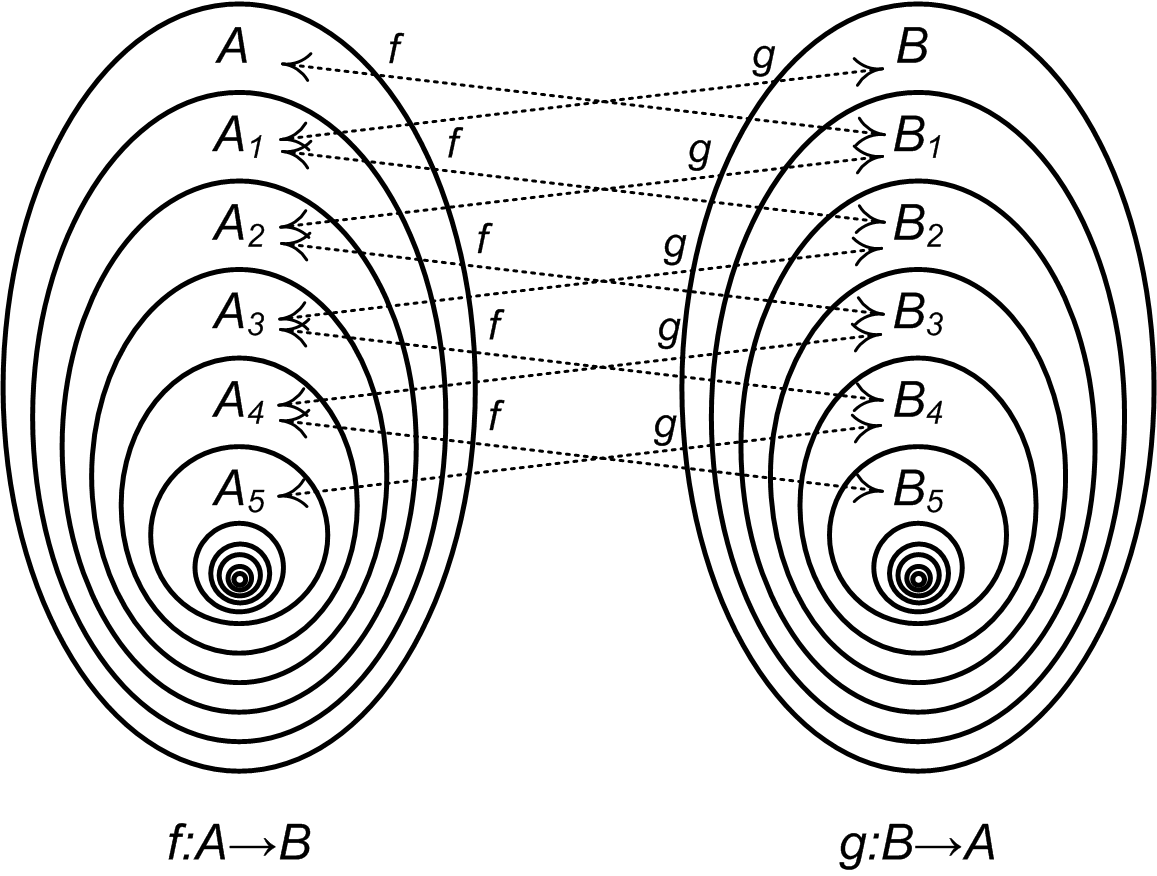
\includegraphics[width=.6\textwidth]{fig/kantorBernstein1}
    \end{center}
\end{frame}

\begin{frame}
    \frametitle{Доказательство теоремы Кантора-Бернштейна}
    
    Пусть $A_0=A$, $A_1=g(B)$, $A_{n+2}=(f\cdot g)(A_n)$. Видно, что $A_{n+1}\subseteq A_n$. Пусть $M_i=A_i\backslash A_{i+1}$. Видно, что существует биекция $f\cdot g:M_{i}\leftrightarrow M_{i+2}$. Справедливо также, что при $i\neq j$ выполняется $M_i\cap M_j=\emptyset$. Обозначим $D=\bigcap_{k\in\mathbb{N}} A_k$. 

    \begin{center}
        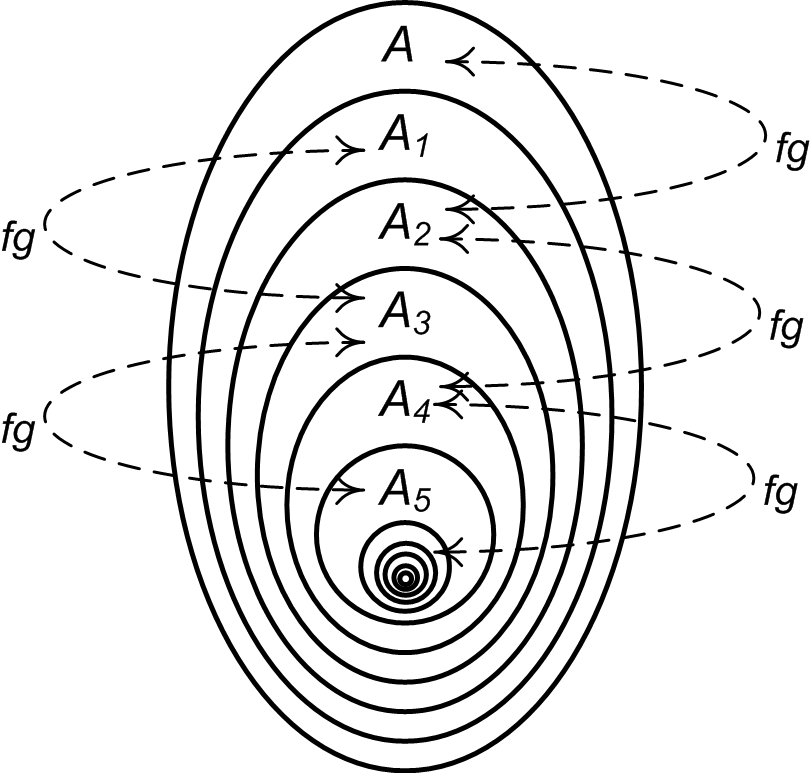
\includegraphics[width=.45\textwidth]{fig/kantorBernstein2}
    \end{center}
\end{frame}

\begin{frame}
    \frametitle{Доказательство теоремы Кантора-Бернштейна}

    Очевидно, что $A_k=(\bigcup_{i\in\mathbb{N},i\geq k}M_i)\cup D$. Определим биективное отображение $h:A\leftrightarrow A_1$:
    \[
    h(a)=
        \begin{cases}
            a,             &\text{если\,} a\in(\bigcup_{i\in\mathbb{N}}M_{2i+1})\cup D\\
            (f\cdot g)(a), &\text{если\,} a\in\bigcup_{i\in\mathbb{N}}M_{2i}.
        \end{cases}
    \]
\end{frame}

\begin{frame}
    \frametitle{Доказательство теоремы Кантора-Бернштейна}

    $h:A\leftrightarrow A_1$.
    \begin{center}
        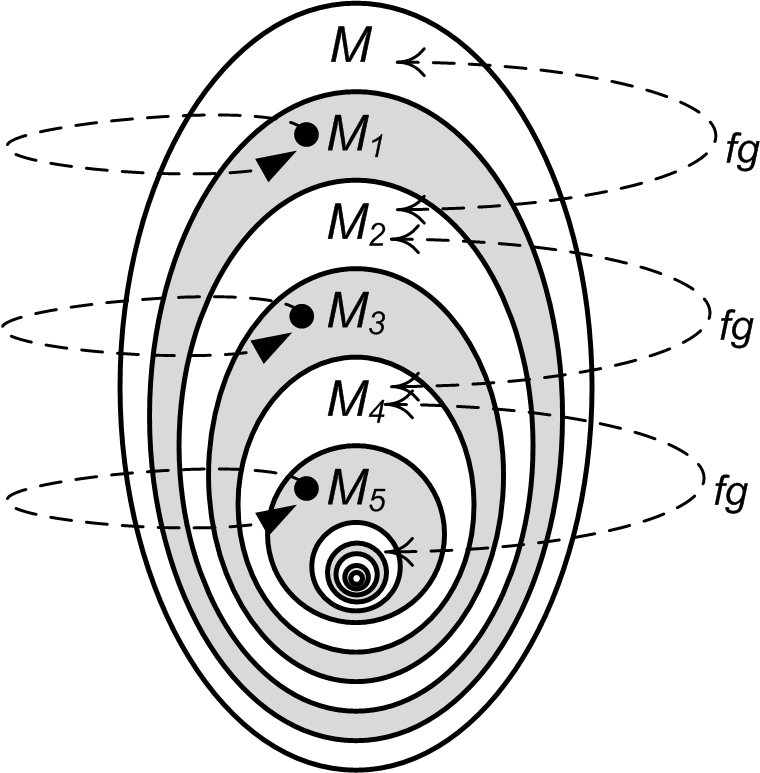
\includegraphics[width=.45\textwidth]{fig/kantorBernstein3}
    \end{center}

    Раз $h$ существует, то $A\sim A_1$, но $A_1\sim B$, следовательно $A\sim B$, то есть $|A|=|B|$.
\end{frame}
    

\begin{frame}
    \frametitle{Отношение мощностей множеств}
    \framesubtitle{Следствие из теоремы Кантора-Бернштейна}
    
    Для любых множеств $A$ и $B$ существует \alert{одна и только одна} из трех возможностей:
    \begin{enumerate}
        \item $|A|=|B|$;
        \item $|A|<|B|$;
        \item $|A|>|B|$.
    \end{enumerate}
\end{frame}


\section{Мощность бесконечных множеств}


\subsection{Кардиналы бесконечных множеств}

\begin{frame}
    \frametitle{Кардиналы бесконечных множеств}

    Известно, что 
    \[|\mathbb{N}|=\aleph_0.\]
    
    Справедливо ли
    \[|\mathbb{N}\times\mathbb{N}|=|\mathbb{N}^2|=\aleph_0^2?\]

    \uncover<2>{
        \alert{Нет}:
        \[|\mathbb{N}\times\mathbb{N}|=|\mathbb{N}^2|=\aleph_0.\]
        
        Т.е.
        \[|\mathbb{N}|=|\mathbb{N}^2|=\aleph_0.\]
    }
\end{frame}

\begin{frame}
    \frametitle{$|\mathbb{N}^2|=|\mathbb{N}|=\aleph_0$}
        
    \begin{center}
        \begin{tabular}{cc}
            \raisebox{-.5\height}{
                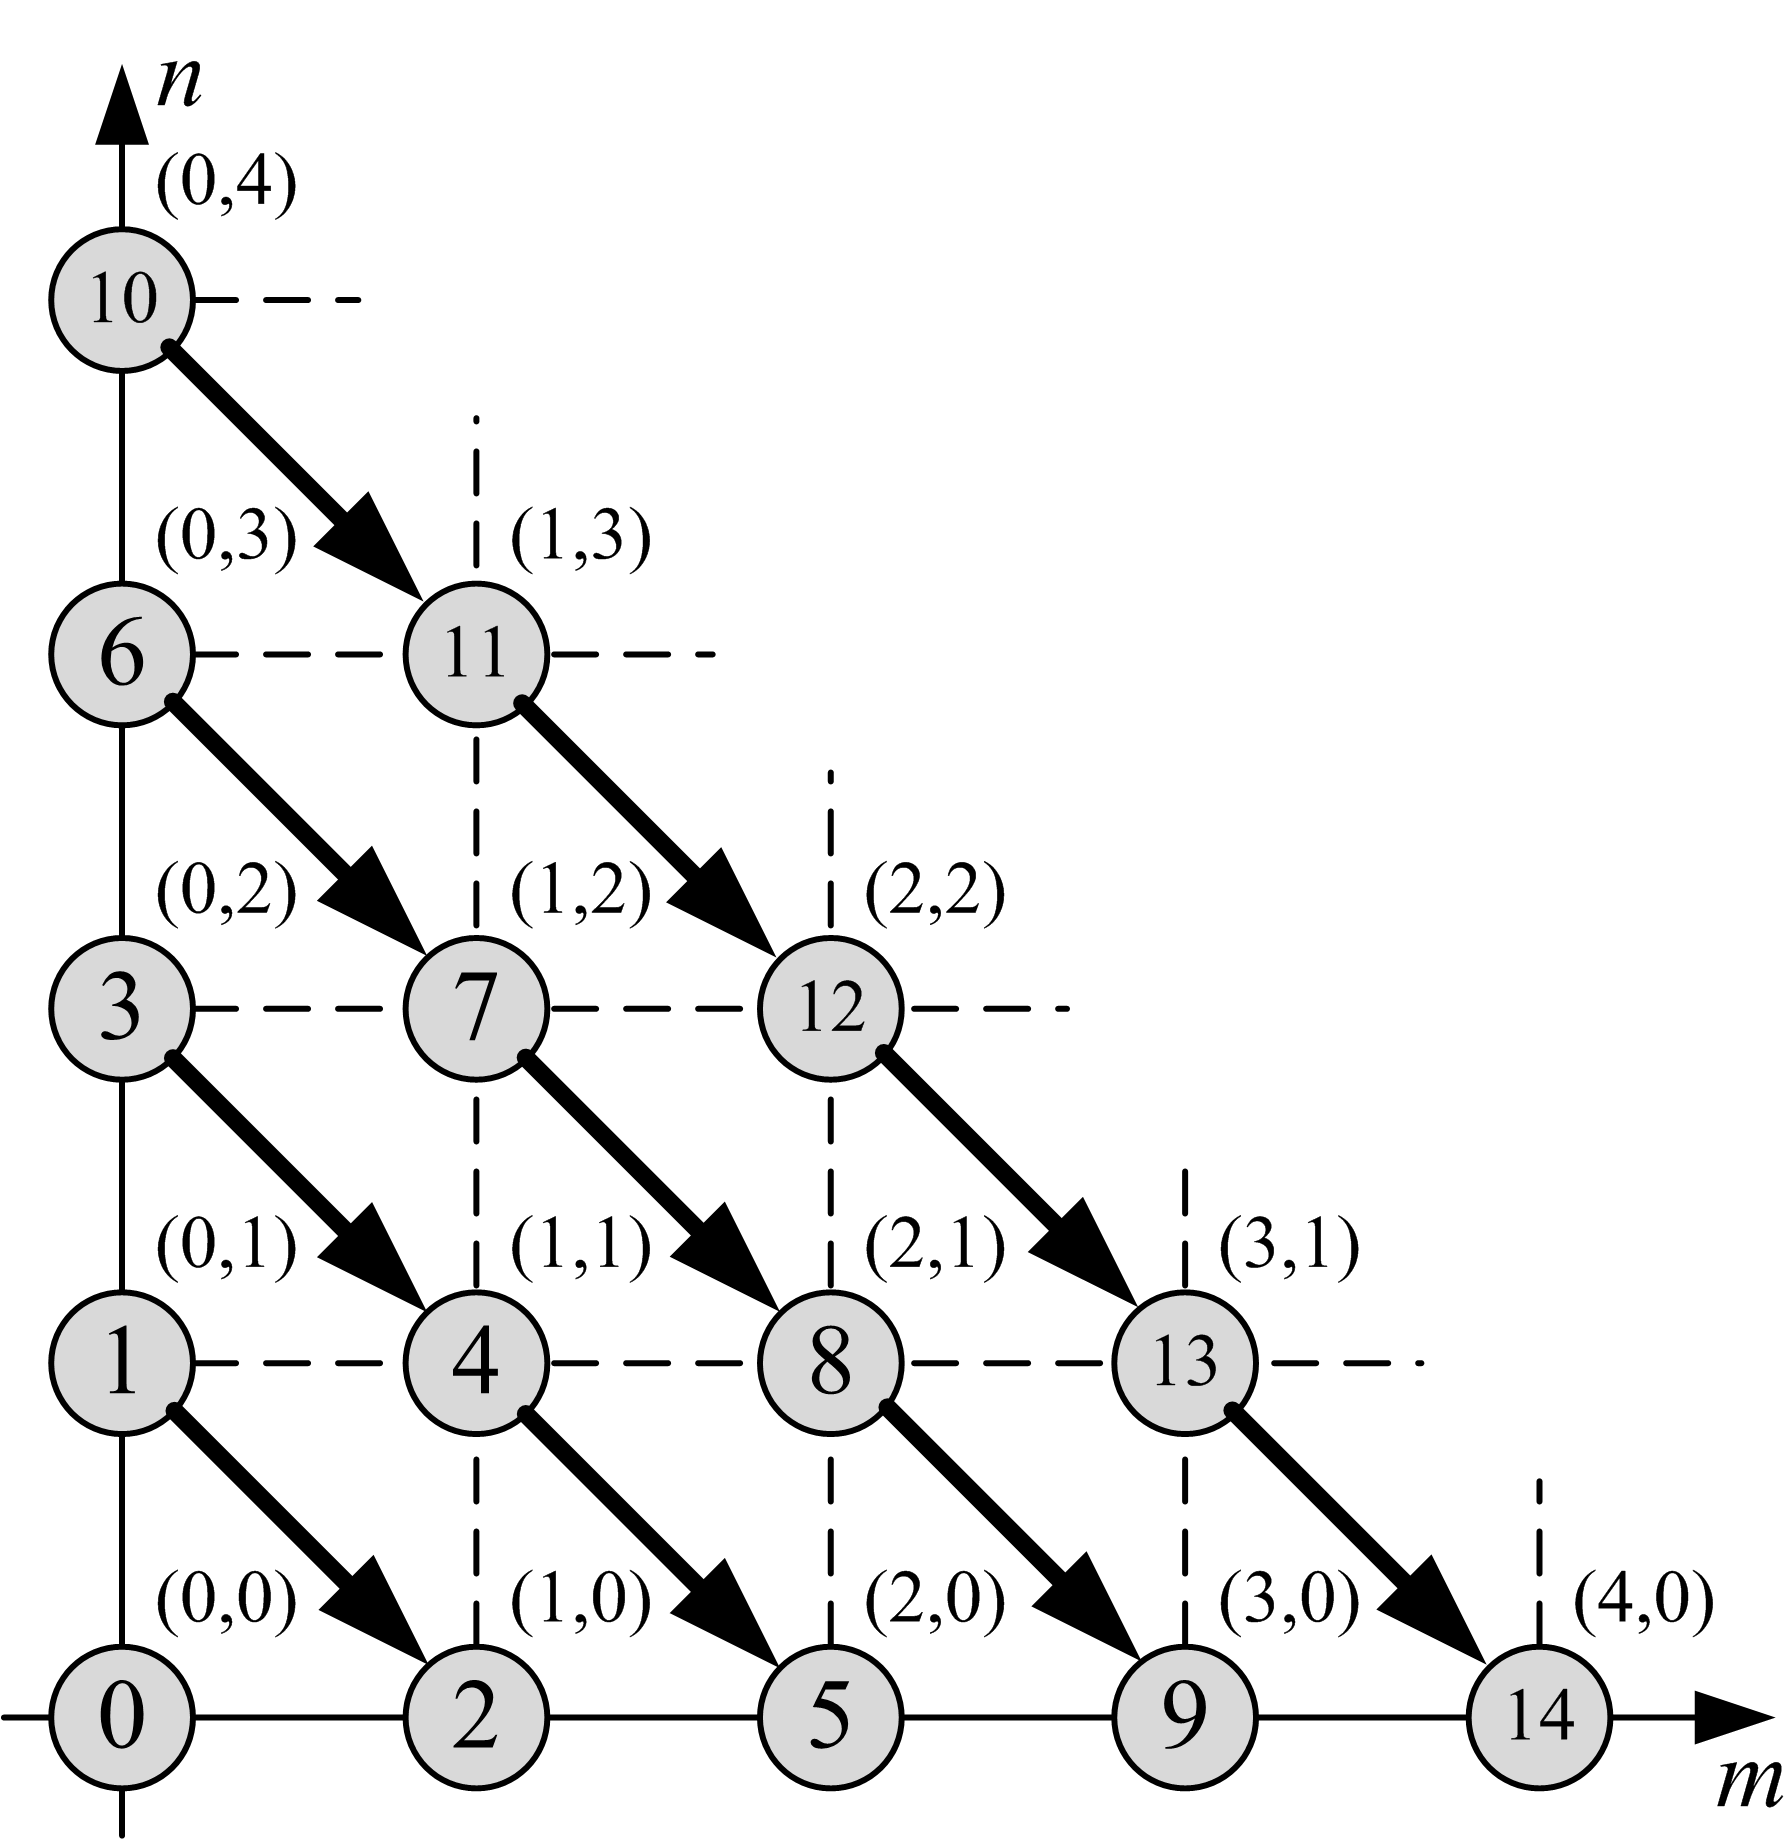
\includegraphics[width=.55\textwidth]{fig/diagonalKantor}
            }
            & $f:\mathbb{N}\leftrightarrow\mathbb{N}^2$
        \end{tabular}
    \end{center}
\end{frame}

\begin{frame}
    \frametitle{Кардиналы бесконечных множеств}
    
    Справедливо также, что:
    \begin{itemize}
        \item $(\mathbb{N}\sim\mathbb{N}^n)\Leftrightarrow (|\mathbb{N}^n|=\aleph_0)$;
        \item $\displaystyle\left(\mathbb{N}\sim\bigcup_{n\in\mathbb{N}}\mathbb{N}^n\right) \Leftrightarrow \left(\left|\bigcup_{n\in\mathbb{N}}\mathbb{N}^n\right|=\aleph_0\right)$.
    \end{itemize}
\end{frame}


\subsection{Есть ли кардиналы больше $\aleph_0$?}

\begin{frame}
    \frametitle{Теорема Кантора}
    
    \begin{theorem}[Кантора]
        Для любого множества $M$ выполняется $|M|<2^{|M|}$.
    \end{theorem}
    \begin{proof}
        Так как для любого $M$ выполняется $|2^M|=2^{|M|}$, то надо показать, что $|M|\leq|2^M|$ и $|M|\neq|2^M|$. Функция $f:M\xrightarrow{\text{в}}2^M$, определенная как $f(x)=\{x\}$, очевидно, инъективна, а тогда справедливо $|M|\leq|2^M|$. Теперь предположим, что $|M|=|2^M|$. Тогда существует биекция $\varphi:M\leftrightarrow 2^M$. Рассмотрим множество $K=\{x|x\in M,x\not\in\varphi(x)\}$. Поскольку $\varphi$ --- биекция и $K\subseteq M$, т.е. $K\in 2^M$, то существует $s\in M$, такое, что $\varphi(s)=K$. Если $s\in K$, то из определения $K$ получаем, что $s\not\in(K=\varphi(k))$. Если $s\not\in K$, то $s\not\in\varphi(s)$ и из определения $K$ следует, что должно выполняться $s\in K$. Противоречие показывает, что биекция $\varphi$ существовать не может.
    \end{proof}
\end{frame}

\begin{frame}
    \frametitle{Кардиналы, больше $\aleph_0$ существуют}
    \framesubtitle{Следствие из теоремы Кантора}
    
    Для бесконечных множеств кардиналы имеют вид: 
    \[
    \resizebox{.5\textwidth}{!}{$\aleph_0, 2^{\aleph_0}, 2^{2^{\aleph_0}}, \ldots$}
    \]
    
    Если $A\sim 2^{\mathbb{N}}$, то множество $A$ называется \alert{континуальным} или \alert{континуумом}: $|A|=2^{\aleph_0}$. Слово континуум означает непрерывный.
\end{frame}

\begin{frame}
    \frametitle{$2^\mathbb{N}\sim 10^\mathbb{N}\sim \mathbb{N}^\mathbb{N}$}
    
    Неравенства $2^\mathbb{N}\leq 10^\mathbb{N}\leq \mathbb{N}^\mathbb{N}$ очевидны. Достаточно показать, что $\mathbb{N}^\mathbb{N}\leq 2^\mathbb{N}$, т.е. существует $\varphi:\mathbb{N}^\mathbb{N}\xrightarrow{\text{в}}2^\mathbb{N}$. Это значит, что $\varphi$ кодирует все возможные бесконечные последовательности натуральных чисел последовательностями из нулей и единиц. Пусть $f\in\mathbb{N}^\mathbb{N}$:
    \[f=f_0,f_1,\ldots,f_n,\ldots\]
    определим последовательность $\varphi(f)\in 2^\mathbb{N}$ так:
    \[
        \varphi(f)=\underbrace{1,1,\ldots,1}_{f_0},0,
        \underbrace{1,1,\ldots,1}_{f_1},0,\ldots,0,
        \underbrace{1,1,\ldots,1}_{f_n},0,\ldots
    \]
    \begin{example}
        Если $\varphi(f)=0,1,1,1,0,0,1,1,1,1,1,0\ldots$, то $f=0,3,0,5,\ldots$
    \end{example}
\end{frame}

\begin{frame}
    \frametitle{$\mathbb{R}\sim [0,1]$}
    \framesubtitle{Отрезок вещественной оси $[0,1]$ называется континуумом}
    
    Доказать, что мощности отрезка $[0,1]$ и интервала $(0,1)$ равны, можно задав биекцию:
    \[
        \varphi(x)=
        \begin{cases}
            x,&\text{если $x\neq 0,x\neq\frac{1}{n},(n\in\mathbb{N},n>0)$},\\
            \frac{1}{2},&\text{если $x=0$},\\
            \frac{1}{3},&\text{если $x=1$},\\
            \frac{1}{n+2},&\text{если $x=\frac{1}{n},n\in\mathbb{N},n>1$}.\\
        \end{cases}
    \]
\end{frame}

\begin{frame}
    \frametitle{$\mathbb{R}\sim [0,1]$}
    
    В свою очередь биекция $\psi(x)=\tan(\pi(x-\frac{1}{2}))$ определяет эквивалентность интервала $(0,1)$ и множества $\mathbb{R}$. Тогда биекция $\psi(\varphi(x))$, $x\in[0,1]$ определяет $[0,1]\sim\mathbb{R}$.
    \begin{center}
        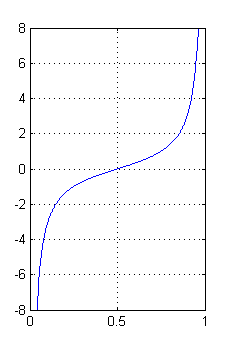
\includegraphics[height=.6\textheight]{fig/tanx}
    \end{center}
\end{frame}

\begin{frame}
    \frametitle{$|\mathbb{R}|=2^{\aleph_0}$}
    
    Любое вещественное число $X$ из $[0,1]$ можно задать в десятичном представлении бесконечной последовательностью:
    \[
        X\equiv(0.a_1a_2\cdots a_n\cdots)_{10},
    \]
    где $n\in\mathbb{N}$ и $a_i\in\{0,\ldots,9\}$. При этом число определяется как
    \[
        X=\sum_{i\geq 1,i\in\mathbb{N}}a_i\cdot \frac{1}{10^i}.
    \]
    
    Видно, что $[0,1]\sim 10^\mathbb{N}$. Исходя из ранее доказанного: $10^\mathbb{N}\sim 2^\mathbb{N}$ и $\mathbb{R}\sim[0,1]$, следует 
    \[
        \mathbb{R}\sim 2^\mathbb{N},
        |\mathbb{R}|=2^{\aleph_0}.
    \]
\end{frame}


\appendix


\begin{frame}
    \frametitle{В заключение}
    
    \begin{itemize}
        \item Мощность множества называется кардиналом.
        \item Кардиналом конечного множества является натуральное число.
        \item Множество натуральных чисел имеет кардинал $|\mathbb{N}|=\aleph_0$.
        \item Кардиналы конечных и бесконечных множеств ведут себя по разному. Например, если $A$ --- конечно, то $|A^2|=|A|^2$, в то время как $|\mathbb{N}^2|=\aleph_0$.
        \item Множество вещественных чисел имеет кардинал $2^{\aleph_0}$.
        \item Кардиналов бесконечных множеств бесконечно много.
    \end{itemize}
    
    Дано более строгое определение мощности. Для углубленного изучения рекомендуются \cite{bib:sudoplatov:discrmath,bib:shaporev:discretemath}.
    
\end{frame}


\begin{frame}[allowframebreaks]{Библиография}
    \bibliographystyle{gost780u}
    \bibliography{./../../bibliobase}
\end{frame}

\end{document}